\documentclass[
11pt, % The default document font size, options: 10pt, 11pt, 12pt
codirector, % Uncomment to add a codirector to the title page
]{charter} 

\usepackage{makecell} %
\usepackage{textcomp} %

% El títulos de la memoria, se usa en la carátula y se puede usar el cualquier lugar del documento con el comando \ttitle
\titulo{Sistema de monitoreo remoto de apiarios} 

% Nombre del posgrado, se usa en la carátula y se puede usar el cualquier lugar del documento con el comando \degreename
%\posgrado{Carrera de Especialización en Sistemas Embebidos} 
\posgrado{Carrera de Especialización en Internet de las Cosas} 
%\posgrado{Carrera de Especialización en Intelegencia Artificial}
%\posgrado{Maestría en Sistemas Embebidos} 
%\posgrado{Maestría en Internet de las cosas}

% Tu nombre, se puede usar el cualquier lugar del documento con el comando \authorname
\autor{Lic. Cynthia Escobar} 

% El nombre del director y co-director, se puede usar el cualquier lugar del documento con el comando \supname y \cosupname y \pertesupname y \pertecosupname
\director{Mg. Ing. Carlos Fontela}
\pertenenciaDirector{FIUBA} 
% FIXME:NO IMPLEMENTADO EL CODIRECTOR ni su pertenencia
\codirector{Esp. Ciro Romero} % para que aparezca en la portada se debe descomentar la opción codirector en el documentclass
\pertenenciaCoDirector{FIUBA}

% Nombre del cliente, quien va a aprobar los resultados del proyecto, se puede usar con el comando \clientename y \empclientename
\cliente{Sr. Enrique Soto}
\empresaCliente{La Agroapícola}

% Nombre y pertenencia de los jurados, se pueden usar el cualquier lugar del documento con el comando \jurunoname, \jurdosname y \jurtresname y \perteunoname, \pertedosname y \pertetresname.
\juradoUno{Nombre y Apellido (1)}
\pertenenciaJurUno{pertenencia (1)} 
\juradoDos{Nombre y Apellido (2)}
\pertenenciaJurDos{pertenencia (2)}
\juradoTres{Nombre y Apellido (3)}
\pertenenciaJurTres{pertenencia (3)}
 
\fechaINICIO{21 de octubre de 2021}    %Fecha de inicio de la cursada de GdP \fechaInicioName
\fechaFINALPlan{8 de diciembre de 2021} 	%Fecha de final de cursada de GdP
\fechaFINALTrabajo{20 de noviembre de 2022}	%Fecha de defensa pública del trabajo final


\begin{document}

\maketitle
\thispagestyle{empty}
\pagebreak


\thispagestyle{empty}
{\setlength{\parskip}{0pt}
\tableofcontents{}
}
\pagebreak


\section*{Registros de cambios}
\label{sec:registro}


\begin{table}[ht]
\label{tab:registro}
\centering
\begin{tabularx}{\linewidth}{@{}|c|X|c|@{}}
\hline
\rowcolor[HTML]{C0C0C0} 
Revisión & \multicolumn{1}{c|}{\cellcolor[HTML]{C0C0C0}Detalles de los cambios realizados} & Fecha      \\ \hline
0      & Creación del documento                                 & 21/10/2021 \\ \hline
1      & Se completa hasta el punto 5 inclusive                 & 01/11/2021 \\ \hline
2      & Se completa hasta el punto 9 inclusive                 & 08/11/2021 \\ \hline
%		  Se puede agregar algo más \newline
%		  En distintas líneas \newline
%		  Así                                                    & dd/mm/aaaa \\ \hline
%3      & Se completa hasta el punto 11 inclusive                & dd/mm/aaaa \\ \hline
%4      & Se completa el plan	                                 & dd/mm/aaaa \\ \hline
\end{tabularx}
\end{table}

\pagebreak



\section*{Acta de constitución del proyecto}
\label{sec:acta}

\begin{flushright}
Buenos Aires, \fechaInicioName
\end{flushright}

\vspace{2cm}

Por medio de la presente se acuerda con la \authorname\hspace{1px} que su Trabajo Final de la \degreename\hspace{1px} se titulará ``\ttitle''. Consistirá esencialmente en el prototipo preliminar de un sistema de medición, visualización y emisión de alertas destinado al monitoreo de apiarios, y tendrá un presupuesto preliminar estimado de 600 hs de trabajo y {\$250000}, con fecha de inicio \fechaInicioName\hspace{1px} y fecha de presentación pública \fechaFinalName.

%50k + 250 $/h * cant horas humanas + 50k (por gastos extras) = 250k

Se adjunta a esta acta la planificación inicial.

\vfill

% Esta parte se construye sola con la información que hayan cargado en el preámbulo del documento y no debe modificarla
\begin{table}[ht]
\centering
\begin{tabular}{ccc}
\begin{tabular}[c]{@{}c@{}}Ariel Lutenberg \\ Director posgrado FIUBA\end{tabular} & \hspace{2cm} & \begin{tabular}[c]{@{}c@{}}\clientename \\ \empclientename \end{tabular} \vspace{2.5cm} \\ 
\multicolumn{3}{c}{\begin{tabular}[c]{@{}c@{}} \supname \\ Director del Trabajo Final\end{tabular}} \vspace{2.5cm} \\
%\begin{tabular}[c]{@{}c@{}}\jurunoname \\ Jurado del Trabajo Final\end{tabular}     &  & \begin{tabular}[c]{@{}c@{}}\jurdosname\\ Jurado del Trabajo Final\end{tabular}  \vspace{2.5cm}  \\
%\multicolumn{3}{c}{\begin{tabular}[c]{@{}c@{}} \jurtresname\\ Jurado del Trabajo Final\end{tabular}} \vspace{.5cm}                                                                     
\end{tabular}
\end{table}




\section{1. Descripción técnica-conceptual del proyecto a realizar}
\label{sec:descripcion}

Las abejas son indispensables en la conservación del ecosistema y en la producción de alimentos gracias al importante papel que juegan como polinizadores en la fertilización y reproducción de las plantas.
% ya que en su afán de alimentarse transportan polen de flor en flor y contribuyen a la fecundación y reproducción de las plantas.

La apicultura es la actividad realizada por el hombre que consiste en la cría y en el cuidado apropiado de las abejas para lograr que sus colonias prosperen y se pueda obtener de ellas para el consumo y/o comercialización: miel, polen, jalea real, propóleo y cera.

Es una actividad noble que a pesar de tener un fin económico trabaja buscando un equilibrio entre la explotación comercial y preservación de las abejas y el medio ambiente.

A pesar de los avances tecnológicos la apicultura sigue siendo una práctica casi artesana ya que el apicultor debe estar muy involucrado en el mantenimiento y cuidado de sus colmenas. Se deben realizar visitas periódicas para controlar la salubridad de las abejas, chequear los niveles de alimentos y el estado general de las colmenas.
Como los apiarios suelen estar instalados lejos de los centros urbanos estas visitas suelen consumir tiempo y recursos, y de no realizar visitas periódicas uno se arriesga a poder perder colmenas.

El objetivo de esta solución es ayudar a minimizar la intervención del apicultor y sus costos asociados al proveerle de una herramienta que le permita monitorear distintas variables de sus colmenas de manera remota.


El monitoreo remoto propuesto se planea realizar a través de la recopilación de datos con los siguientes instrumentos instalados dentro de la cámara de cría de una colmena de abejas europeas (\textit{Apis mellifera}):
\begin{itemize}
\item sensor de temperatura. 
\item sensor de humedad.
\item sensor de sonido.
\item sensor de inclinación (giróscopo).
\end{itemize}


En la figura 1 se presenta el diagrama en bloques del sistema que representa los distintos componentes que trabajarán en conjunto para recopilar datos y permitir controlar remotamente el estado de las colmenas.

\begin{figure}[htpb]
\centering 
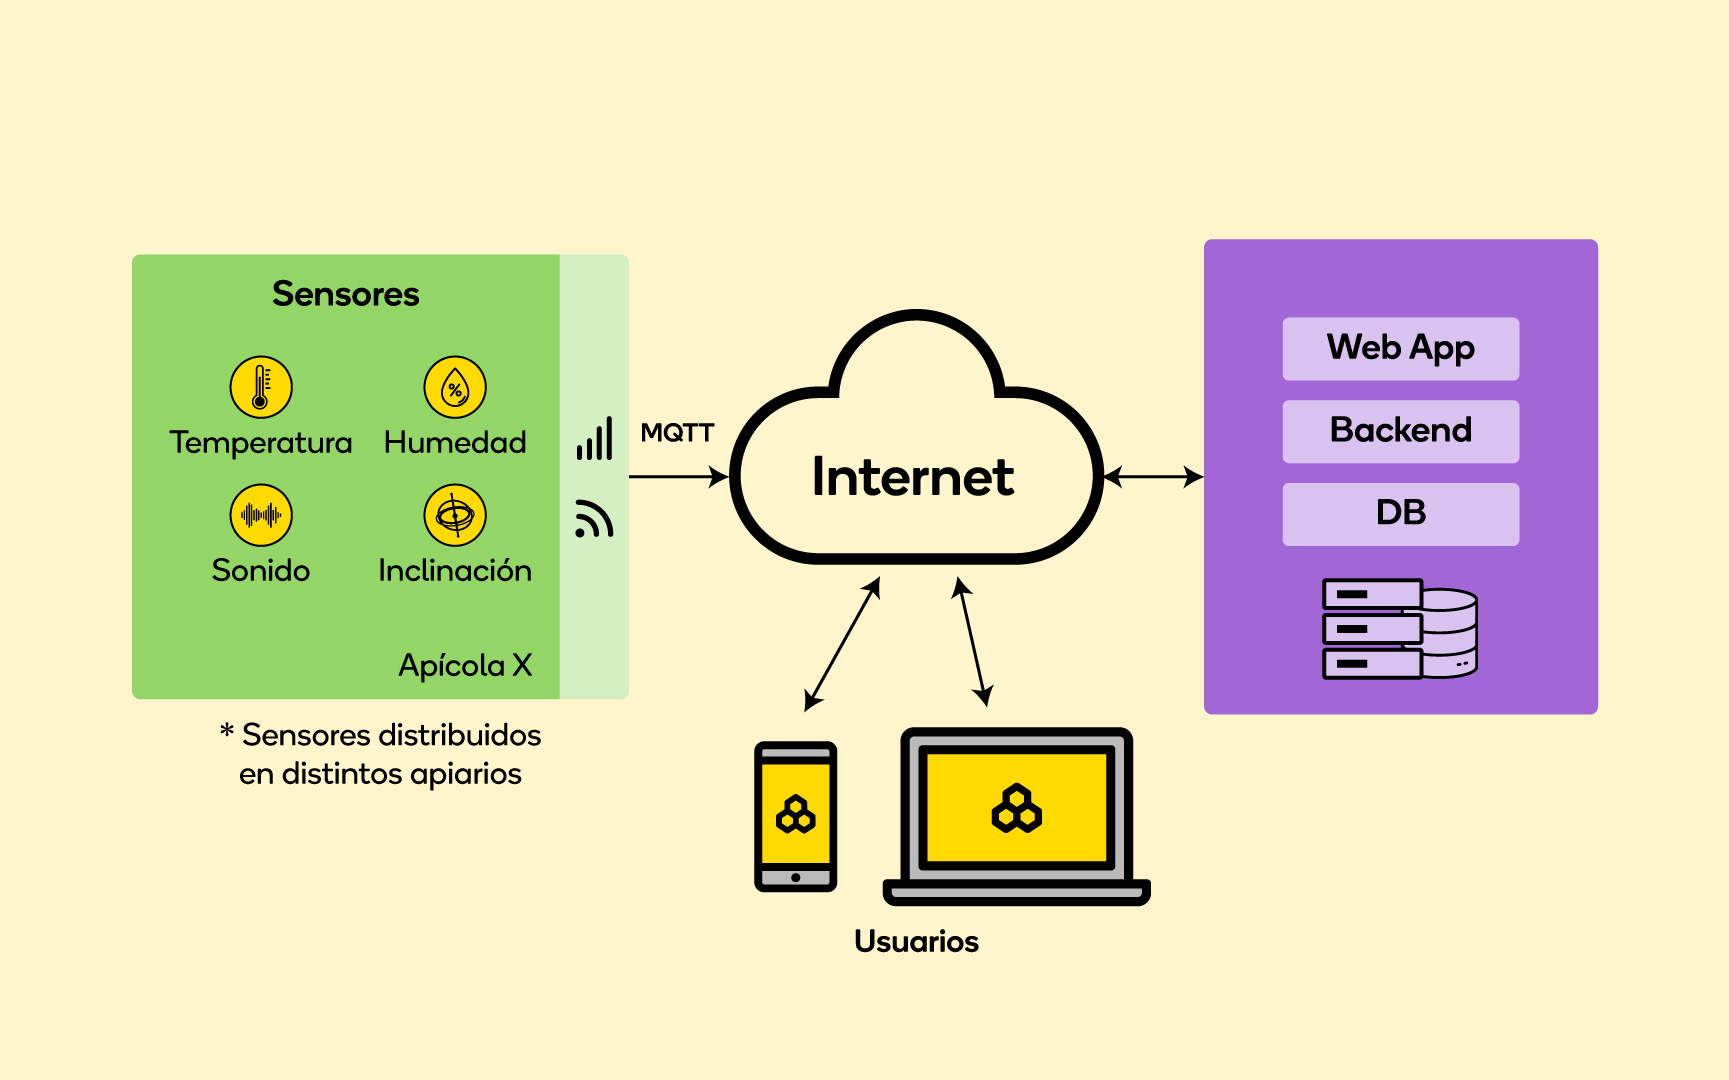
\includegraphics[width=1\textwidth]{./Figuras/diagBloquesPropio.jpg}
\caption{Diagrama en bloques del sistema.}
\label{fig:diagBloques}
\end{figure}



La solución se compone de las siguientes partes:
\begin{itemize}
\item medición de la temperatura, de la humedad y del sonido en el interior de la cámara de cría y de su inclinación.
%\item transporte de los datos
\item lógica de procesamiento y persistencia de datos.
\item visualización de métricas y alarmas.
\end{itemize}

Se propone que las mediciones sean recolectadas en los apiarios, transmitidas a un broker MQTT para finalmente ser enviadas a un servicio backend para su procesamiento, análisis y persistencia.
También se contempla el desarrollo de un frontend para que el usuario pueda:
\begin{itemize}
\item acceder a la visualización de las métricas y alertas.
\item acceder a un dashboard de administración y configuración.
\end{itemize}
Desde este frontend se espera que el usuario pueda establecer los thresholds de aceptabilidad para cada una de las métricas, así como la configuración de las acciones a tomar luego del disparo de una alarma de sistema.

%\vspace{25px}
\section{2. Identificación y análisis de los interesados}
\label{sec:interesados}

\begin{table}[ht]
%\caption{Identificación de los interesados}
%\label{tab:interesados}
\begin{tabularx}{\columnwidth}{@{}|l|X|l|l|@{}}
\hline
\rowcolor[HTML]{C0C0C0} 
Rol           & Nombre y Apellido & Organización 	& Puesto 	\\ \hline
%Auspiciante   &        -          &        -      	&     -   	\\ \hline
Cliente       & \clientename      &\empclientename	&    -   	\\ \hline
%Impulsor      &                   &              	&        	\\ \hline
Responsable   & \authorname       & FIUBA        	& Alumno 	\\ \hline
Colaboradores &      Sr. Anibal Taverna             & MAGyP            	&     Coordinación de Apicultura   	\\ \hline
Orientadores  & \makecell[l]{\supname \\ \cosupname}	       & \pertesupname 	& \makecell[l]{Director Trabajo final\\Codirector Trabajo final} \\ \hline
%Equipo        & -  &  - & - \\ \hline
%Opositores    &                   &              	&        	\\ \hline
Usuario final & Apicultores               &       -       	&     -   	\\ \hline
\end{tabularx}
\end{table}

\begin{itemize}
\item Cliente: quien dará la aprobación del producto si las pruebas demuestran una mejora en la actividad.
\item Responsable: quien estará a cargo del análisis, planificación y desarrollo del proyecto.
\item Colaborador: una autoridad en la actividad que es fuente de información y consejo tanto en lo técnico como en lo práctico.
\item Orientador: quien en base a su extensa experiencia colaborará en la revisión y planificación del proyecto, y será una guía de referencia para el Responsable.
\item Usuario Final: aquella persona cuya actividad es la apicultura y colaborará con las pruebas.
\end{itemize}

\section{3. Propósito del proyecto}
\label{sec:proposito}

El propósito de este proyecto es colaborar con el cuidado de las colonias de abejas a cargo de apicultores y mejorar la productividad de la actividad poniendo en marcha un sistema que recabe información de las condiciones internas de la cámara de cría. De esta forma permite detectar de manera temprana enfermedades, accidentes y enjambrazones (abandono de la reina de la colmena para crear una nueva colonia)  minimizando la pérdida de colmenas con una intervención mínima del apicultor.

\section{4. Alcance del proyecto}
\label{sec:alcance}

El alcance de este proyecto incluye: 
\begin{itemize}
\item desarrollo de una aplicación backend que se encargue de:
	\begin{itemize}
	\item gestión de usuarios, configuraciones de thresholds, alertas, notificaciones.
	\item procesamiento de las mediciones capturadas.
	\item gestión de altas, bajas y modificaciones de nuevos apiarios.
	\end{itemize}
\item desarrollo de una aplicación web que permita visualizar las métricas y acceder a la configuración del sistema.
\item desarrollo de un prototipo que integre los sensores instalados en el interior de la cámara de cría, con capacidad de conectarse a internet para el envío de los datos a un servidor.
\end{itemize}

El presente proyecto no incluye:

\begin{itemize}
\item la confección de la placa PCB.
\item instalación de red wifi.
\item instalación y configuración de servidor y base de datos.
\end{itemize}

\section{5. Supuestos del proyecto}
\label{sec:supuestos}

Para el desarrollo del presente proyecto se supone que:

\begin{itemize}
\item se tendrá acceso a una red WiFi o a la red GSM/GPRS en el apiario.
\item se simularán los sensores con distintas configuraciones ambientales.
\item se contará con la colaboración del cliente para la evaluación de las pruebas.
\item se contará con el tiempo suficiente para realizar las distintas tareas.
\item se dispondrá de una colmena de abejas europeas para realizar pruebas.
\item el dispositivo que vivirá dentro de la colmena podrá transmitir información a pesar de ser propolizado.
\item la presencia del dispositivo no impactará en la rutina de la colonia ni del apicultor.
\end{itemize}

\section{6. Requerimientos}
\label{sec:requerimientos}

%Los requerimientos deben numerarse y de ser posible estar agruparlos por afinidad, por ejemplo:

\begin{enumerate}
	\item Requerimientos del nodo de medición
		\begin{enumerate}
			\item deberá estar protegido para evitar que las abejas recubran su superficie con propóleo (propolización) que pueda afectar su funcionamiento.
			\item deberá medir la temperatura en un rago de 0 \textdegree{}C--50 \textdegree{}C.
			\item deberá medir la humedad en un rango de 0--100\%.
			\item deberá medir el sonido en un rango de 100 Hz--10kHz.
			\item deberá medir la posición haciendo uso de un giroscopio y acelerómetro.
			\item realizar las capturas cada 3 minutos.
			\item deberá contar con tecnología GSM/GPRS para la conexión a la red de datos.
			\item deberá tener un parámetro que lo identifique inequívocamente.
			\item deberá conectarse a un servidor externo para obtener la hora.
			\item deberá sincronizar el reloj interno para que independientemente de la hora de impacto en el backend la hora de medición sea confiable.
			\item deberá contar con almacenamiento local (SD).
			\item deberá tener capacidad para reintentar el envío de métricas ante pérdida de conexión.
		\end{enumerate}
	\item Requerimientos de seguridad
		\begin{enumerate}
			\item autenticación de los nodos y encriptación de los datos utilizando Mutual TLS.
			\item acceso a la aplicación web con usuario y contraseña.
		\end{enumerate}
	\item Requerimientos de la aplicación backend
		\begin{enumerate}
			\item deberá enviar un alerta al usuario cuando detecte que la posición vertical de la colmena ha variado.
			\item deberá enviar un alerta al detectar que la temperatura en la cámara de cría varía por fuera de los 34\textdegree{}C--36\textdegree{}C.
			\item deberá enviar un alerta al usuario cuando detecte un cambio brusco de la temperatura en la cámara de cría.
			\item deberá emitir un alerta cuando se detecte que la humedad a superado el 14\%.
			\item deberá mantener un histórico de las métricas de hasta 1 mes.
		\end{enumerate}
	\item Requerimientos de la aplicación web
		\begin{enumerate}		
			\item deberá mostrar la temperatura en una serie temporal.
			\item deberá mostrar la humedad en una serie temporal.
			\item deberá mostrar el sonido en una serie temporal.	
			\item deberá mostrar la posicion en una serie temporal.
			\item deberá mostrar la configuración personal del usuario.
			\item deberá mostrar un histórico de los alertas.
		\end{enumerate}
	\item Requerimientos de documentación
		\begin{enumerate}
			\item se debe generar un documento de casos de prueba.
			\item se debe generar un manual de usuario.
		\end{enumerate}	
\end{enumerate}


\section{7. Historias de usuarios (\textit{Product backlog})}
\label{sec:backlog}

Se eligió una escala basada en la serie Fibonacci desde 1 a 13.
La ponderación de estas historias se realizó teniendo en cuenta la dificultad y complejidad en resolverlas:

\begin{tabular}{|c|c|}
\hline
\rowcolor[HTML]{C0C0C0} 
Dificultad & Ponderación \\ \hline
Baja      & 1 \\ \hline
Media      & 3 \\ \hline
Alta      & 5 \\ \hline
\end{tabular}

\begin{tabular}{|c|c|}
\hline
\rowcolor[HTML]{C0C0C0} 
Complejidad & Ponderación \\ \hline
Baja      & 1 \\ \hline
Media      & 5 \\ \hline
Alta      & 8 \\ \hline
\end{tabular}

\begin{tabular}{|c|c|c|}
\hline
\rowcolor[HTML]{C0C0C0} 
Dificultad & Complejidad & Story Point \\ \hline
1 & 1 & 3 \\ \hline
1 & 5 & 5 \\ \hline
1 & 8 & 8 \\ \hline
3 & 1 & 5 \\ \hline
3 & 5 & 8 \\ \hline
3 & 8 & 13 \\ \hline
5 & 1 & 5 \\ \hline
5 & 5 & 8 \\ \hline
5 & 8 & 13 \\ \hline
\end{tabular}

A continuación se presentan las historias de usuarios:
\begin{itemize}
	\item como usuario quiero acceder a la aplicación web con mi correo y contraseña. Dificultad: 5. Complejidad: 8. SP: 13.
	\item como usuario quiero modificar mi configuración. Dificultad: 5. Complejidad: 3. SP: 8.
	\item como apicultor quiero poder visualizar la temperatura de cualquiera de mis colmenas. Dificultad: 3. Complejidad: 5. SP: 8.
	\item como apicultor quiero poder recibir un alerta si la temperatura fluctúa fuera de los 34\textdegree{}C--36\textdegree{}C. Dificultad: 1. Complejidad: 5. SP: 5.
	\item como apicultor quiero poder visualizar la humedad de cualquiera de mis colmenas. Dificultad: 3. Complejidad: 5. SP: 8.
	\item como apicultor quiero poder recibir un alerta si la humedad fluctúa por sobre el 14 \%. Dificultad: 1. Complejidad: 5. SP: 5.
	\item como apicultor quiero poder visualizar la posición de cualquiera de mis colmenas. Dificultad: 3. Complejidad: 5. SP: 8.
	\item como apicultor quiero poder recibir un alerta si la posición vertical de la colmena ha variado. Dificultad: 1. Complejidad: 5. SP: 5.
	\item como apicultor quiero poder acceder al histórico de alertas. Dificultad: 3. Complejidad: 5. SP: 8.
	\item como investigador quiero poder acceder al histórico de cualquiera de las métricas. Dificultad: 5. Complejidad: 5. SP: 8.
\end{itemize}

\section{8. Entregables principales del proyecto}
\label{sec:entregables}

Los entregables del proyecto son:

\begin{itemize}
	\item manual de usuario.
	\item diagrama esquemático de la solución.
	\item prototipo funcional.
	\item informes de avance y final del proyecto.
	\item presentación.
\end{itemize}

\section{9. Desglose del trabajo en tareas}
\label{sec:wbs}

\begin{enumerate}
\item Planificación general (50 hs)
	\begin{enumerate}
	\item investigación previa sobre la actividad (20 hs).
	\item búsqueda de colaboradores y clientes (10 hs).
	\item charlas informativas con colaboradores (10 hs).
	\item definición de alcances y requerimientos (10 hs).
	\end{enumerate}
\item Aplicación backend (110 hs)
	\begin{enumerate}
	\item diseño de modelo de datos (10 hs).
	\item creación de certificados (10 hs).
	\item diseño y construcción de la aplicación (50 hs).
	\item pruebas unitarias (30 hs).
	\item pruebas de integración (10 hs).
	\end{enumerate}
\item Aplicación web (103 hs)
	\begin{enumerate}
	\item maquetado (12 hs).
	\item visualización de métricas (20 hs).
	\item visualización de alertas (20 hs).
	\item gestión de configuración (15 hs).
	\item gestión de usuarios (10 hs).
	\item pruebas de visualización de métricas (8 hs).
	\item pruebas de visualización de alertas (8 hs).
	\item pruebas de integración (10 hs).
	\end{enumerate}
\item Desarrollo del prototipo (53 hs)
	\begin{enumerate}
		\item análisis y selección de sensor de temperatura (3 hs).
		\item análisis y selección de sensor de humedad (3 hs).
		\item análisis y selección de sensor de sonido (4 hs).
		\item análisis y selección de sensor de posición (3 hs).	
		\item instalación y protección de nodo de sensores (10 hs).
		\item investigación sobre microcontroladores disponibles (10 hs).
		\item integración de componentes (20 hs).
	\end{enumerate}
\item Firmware de prototipo (179 hs)
	\begin{enumerate}
		\item diseño arquitectura (12 hs).
		\item programación de giroscopio y acelerómetro (15 hs).		
		\item estudio y programación del módulo GSM/GPRS (30 hs).
		\item sincronización reloj interno (5 hs).
		\item estudio de Mutual TLS y creación de certificados (12 hs).
		\item manipulación de datos (25 hs).
		\item desarrollo de la comunicación utilizando Mutual TLS, contemplando reintentos (35 hs).
		\item pruebas unitarias (30 hs)
		\item prubas de integración (15 hs).
	\end{enumerate}
\item Documentación (95 hs)
	\begin{enumerate}
		\item elaboración de manual de pruebas (10 hs).
		\item elaboración del manual de usuario (15 hs).
		\item elaboración del informe de avance (30 hs).		
		\item elaboración de la memoria técnica (40 hs).
	\end{enumerate}
\item Cierre (50 hs)
	\begin{enumerate}
		\item elaboración del informe final (30 hs).	
		\item elaboración de la presentación (20 hs).
	\end{enumerate}
\end{enumerate}

Cantidad total de horas: (640 hs)

\section{10. Diagrama de Activity On Node}
\label{sec:AoN}

\begin{consigna}{red}
Armar el AoN a partir del WBS definido en la etapa anterior. 

%La figura \ref{fig:AoN} fue elaborada con el paquete latex tikz y pueden consultar la siguiente referencia \textit{online}:

%\url{https://www.overleaf.com/learn/latex/LaTeX_Graphics_using_TikZ:_A_Tutorial_for_Beginners_(Part_3)\%E2\%80\%94Creating_Flowcharts}

\end{consigna}

\begin{figure}[htpb]
\centering 
\includegraphics[width=.8\textwidth]{./Figuras/AoN.png}
\caption{Diagrama en \textit{Activity on Node}}
\label{fig:AoN}
\end{figure}

Indicar claramente en qué unidades están expresados los tiempos.
De ser necesario indicar los caminos semicríticos y analizar sus tiempos mediante un cuadro.
Es recomendable usar colores y un cuadro indicativo describiendo qué representa cada color, como se muestra en el siguiente ejemplo:



\section{11. Diagrama de Gantt}
\label{sec:gantt}

\begin{consigna}{red}

Existen muchos programas y recursos \textit{online} para hacer diagramas de gantt, entre los cuales destacamos:

\begin{itemize}
\item Planner
\item GanttProject
\item Trello + \textit{plugins}. En el siguiente link hay un tutorial oficial: \\ \url{https://blog.trello.com/es/diagrama-de-gantt-de-un-proyecto}
\item Creately, herramienta online colaborativa. \\\url{https://creately.com/diagram/example/ieb3p3ml/LaTeX}
\item Se puede hacer en latex con el paquete \textit{pgfgantt}\\ \url{http://ctan.dcc.uchile.cl/graphics/pgf/contrib/pgfgantt/pgfgantt.pdf}
\end{itemize}

Pegar acá una captura de pantalla del diagrama de Gantt, cuidando que la letra sea suficientemente grande como para ser legible. 
Si el diagrama queda demasiado ancho, se puede pegar primero la ``tabla'' del Gantt y luego pegar la parte del diagrama de barras del diagrama de Gantt.

Configurar el software para que en la parte de la tabla muestre los códigos del EDT (WBS).\\
Configurar el software para que al lado de cada barra muestre el nombre de cada tarea.\\
Revisar que la fecha de finalización coincida con lo indicado en el Acta Constitutiva.

En la figura \ref{fig:gantt}, se muestra un ejemplo de diagrama de gantt realizado con el paquete de \textit{pgfgantt}. En la plantilla pueden ver el código que lo genera y usarlo de base para construir el propio.

\begin{figure}[htbp]
\begin{center}
\begin{ganttchart}{1}{12}
  \gantttitle{2020}{12} \\
  \gantttitlelist{1,...,12}{1} \\
  \ganttgroup{Group 1}{1}{7} \\
  \ganttbar{Task 1}{1}{2} \\
  \ganttlinkedbar{Task 2}{3}{7} \ganttnewline
  \ganttmilestone{Milestone o hito}{7} \ganttnewline
  \ganttbar{Final Task}{8}{12}
  \ganttlink{elem2}{elem3}
  \ganttlink{elem3}{elem4}
\end{ganttchart}
\end{center}
\caption{Diagrama de gantt de ejemplo}
\label{fig:gantt}
\end{figure}


\begin{landscape}
\begin{figure}[htpb]
\centering 
\includegraphics[height=.85\textheight]{./Figuras/Gantt-2.png}
\caption{Ejemplo de diagrama de Gantt rotado}
\label{fig:diagGantt}
\end{figure}

\end{landscape}

\end{consigna}


\section{12. Presupuesto detallado del proyecto}
\label{sec:presupuesto}

\begin{consigna}{red}
Si el proyecto es complejo entonces separarlo en partes:
\begin{itemize}
	\item Un total global, indicando el subtotal acumulado por cada una de las áreas.
	\item El desglose detallado del subtotal de cada una de las áreas.
\end{itemize}

IMPORTANTE: No olvidarse de considerar los COSTOS INDIRECTOS.

\end{consigna}

\begin{table}[htpb]
\centering
\begin{tabularx}{\linewidth}{@{}|X|c|r|r|@{}}
\hline
\rowcolor[HTML]{C0C0C0} 
\multicolumn{4}{|c|}{\cellcolor[HTML]{C0C0C0}COSTOS DIRECTOS} \\ \hline
\rowcolor[HTML]{C0C0C0} 
Descripción &
  \multicolumn{1}{c|}{\cellcolor[HTML]{C0C0C0}Cantidad} &
  \multicolumn{1}{c|}{\cellcolor[HTML]{C0C0C0}Valor unitario} &
  \multicolumn{1}{c|}{\cellcolor[HTML]{C0C0C0}Valor total} \\ \hline
 &
  \multicolumn{1}{c|}{} &
  \multicolumn{1}{c|}{} &
  \multicolumn{1}{c|}{} \\ \hline
 &
  \multicolumn{1}{c|}{} &
  \multicolumn{1}{c|}{} &
  \multicolumn{1}{c|}{} \\ \hline
\multicolumn{1}{|l|}{} &
   &
   &
   \\ \hline
\multicolumn{1}{|l|}{} &
   &
   &
   \\ \hline
\multicolumn{3}{|c|}{SUBTOTAL} &
  \multicolumn{1}{c|}{} \\ \hline
\rowcolor[HTML]{C0C0C0} 
\multicolumn{4}{|c|}{\cellcolor[HTML]{C0C0C0}COSTOS INDIRECTOS} \\ \hline
\rowcolor[HTML]{C0C0C0} 
Descripción &
  \multicolumn{1}{c|}{\cellcolor[HTML]{C0C0C0}Cantidad} &
  \multicolumn{1}{c|}{\cellcolor[HTML]{C0C0C0}Valor unitario} &
  \multicolumn{1}{c|}{\cellcolor[HTML]{C0C0C0}Valor total} \\ \hline
\multicolumn{1}{|l|}{} &
   &
   &
   \\ \hline
\multicolumn{1}{|l|}{} &
   &
   &
   \\ \hline
\multicolumn{1}{|l|}{} &
   &
   &
   \\ \hline
\multicolumn{3}{|c|}{SUBTOTAL} &
  \multicolumn{1}{c|}{} \\ \hline
\rowcolor[HTML]{C0C0C0}
\multicolumn{3}{|c|}{TOTAL} &
   \\ \hline
\end{tabularx}%
\end{table}


\section{13. Gestión de riesgos}
\label{sec:riesgos}

\begin{consigna}{red}
a) Identificación de los riesgos (al menos cinco) y estimación de sus consecuencias:
 
Riesgo 1: detallar el riesgo (riesgo es algo que si ocurre altera los planes previstos de forma negativa)
\begin{itemize}
	\item Severidad (S): mientras más severo, más alto es el número (usar números del 1 al 10).\\
	Justificar el motivo por el cual se asigna determinado número de severidad (S).
	\item Probabilidad de ocurrencia (O): mientras más probable, más alto es el número (usar del 1 al 10).\\
	Justificar el motivo por el cual se asigna determinado número de (O). 
\end{itemize}   

Riesgo 2:
\begin{itemize}
	\item Severidad (S): 
	\item Ocurrencia (O):
\end{itemize}

Riesgo 3:
\begin{itemize}
	\item Severidad (S): 
	\item Ocurrencia (O):
\end{itemize}


b) Tabla de gestión de riesgos:      (El RPN se calcula como RPN=SxO)

\begin{table}[htpb]
\centering
\begin{tabularx}{\linewidth}{@{}|X|c|c|c|c|c|c|@{}}
\hline
\rowcolor[HTML]{C0C0C0} 
Riesgo & S & O & RPN & S* & O* & RPN* \\ \hline
       &   &   &     &    &    &      \\ \hline
       &   &   &     &    &    &      \\ \hline
       &   &   &     &    &    &      \\ \hline
       &   &   &     &    &    &      \\ \hline
       &   &   &     &    &    &      \\ \hline
\end{tabularx}%
\end{table}

Criterio adoptado: 
Se tomarán medidas de mitigación en los riesgos cuyos números de RPN sean mayores a...

Nota: los valores marcados con (*) en la tabla corresponden luego de haber aplicado la mitigación.

c) Plan de mitigación de los riesgos que originalmente excedían el RPN máximo establecido:
 
Riesgo 1: plan de mitigación (si por el RPN fuera necesario elaborar un plan de mitigación).
  Nueva asignación de S y O, con su respectiva justificación:
  - Severidad (S): mientras más severo, más alto es el número (usar números del 1 al 10).
          Justificar el motivo por el cual se asigna determinado número de severidad (S).
  - Probabilidad de ocurrencia (O): mientras más probable, más alto es el número (usar del 1 al 10).
          Justificar el motivo por el cual se asigna determinado número de (O).

Riesgo 2: plan de mitigación (si por el RPN fuera necesario elaborar un plan de mitigación).
 
Riesgo 3: plan de mitigación (si por el RPN fuera necesario elaborar un plan de mitigación).

\end{consigna}


\section{14. Gestión de la calidad}
\label{sec:calidad}

\begin{consigna}{red}
Para cada uno de los requerimientos del proyecto indique:
\begin{itemize} 
\item Req \#1: copiar acá el requerimiento.

\begin{itemize}
	\item Verificación para confirmar si se cumplió con lo requerido antes de mostrar el sistema al cliente. Detallar 
	\item Validación con el cliente para confirmar que está de acuerdo en que se cumplió con lo requerido. Detallar  
\end{itemize}

\end{itemize}

Tener en cuenta que en este contexto se pueden mencionar simulaciones, cálculos, revisión de hojas de datos, consulta con expertos, mediciones, etc.  Las acciones de verificación suelen considerar al entregable como ``caja blanca'', es decir se conoce en profundidad su funcionamiento interno.  En cambio, las acciones de validación suelen considerar al entregable como ``caja negra'', es decir, que no se conocen los detalles de su funcionamiento interno.

\end{consigna}

\section{15. Procesos de cierre}    
\label{sec:cierre}

\begin{consigna}{red}
Establecer las pautas de trabajo para realizar una reunión final de evaluación del proyecto, tal que contemple las siguientes actividades:

\begin{itemize}
	\item Pautas de trabajo que se seguirán para analizar si se respetó el Plan de Proyecto original:
	 - Indicar quién se ocupará de hacer esto y cuál será el procedimiento a aplicar. 
	\item Identificación de las técnicas y procedimientos útiles e inútiles que se emplearon, y los problemas que surgieron y cómo se solucionaron:
	 - Indicar quién se ocupará de hacer esto y cuál será el procedimiento para dejar registro.
	\item Indicar quién organizará el acto de agradecimiento a todos los interesados, y en especial al equipo de trabajo y colaboradores:
	  - Indicar esto y quién financiará los gastos correspondientes.
\end{itemize}

\end{consigna}


\end{document}
